\documentclass{article}
\linespread{1.3}
\usepackage[margin=50pt]{geometry}
\usepackage{amsmath, amsthm, amssymb, amsthm, tikz, fancyhdr, float, graphicx, spverbatim, systeme}
\pagestyle{fancy}
\renewcommand{\headrulewidth}{0pt}
\newcommand{\changefont}{\fontsize{15}{15}\selectfont}

\fancypagestyle{firstpageheader}{
  \fancyhead[R]{
    \changefont
    \parbox[t]{4cm}{
      Michael Huang\\
      EN.625.740.81\\
      Homework 4
    }
  }
}

\begin{document}

\thispagestyle{firstpageheader}
{\Large 

\section*{1.}
Fisher's linear discriminant is 
\[
  \hat{\mathbf{w}}^* = \text{arg} \max_{\hat{\mathbf{w}}} J(\hat{\mathbf{w}}) = \text{arg} \max_{\hat{\mathbf{w}}} \frac{\hat{\mathbf{w}}^T \mathbf{S}_b \hat{\mathbf{w}}}{\hat{\mathbf{w}}^T \mathbf{S}_w \hat{\mathbf{w}}}
\]
where \(\mathbf{S}_b = (\mathbf{m_1} - \mathbf{m_2}) (\mathbf{m_1} - \mathbf{m_2})^T\) and \(\mathbf{S}_w = \sum_j \sum_\alpha (\mathbf{x}_\alpha - \mathbf{m}_j) (\mathbf{x}_\alpha - \mathbf{m}_j)^T\)

\subsection*{(a)} 
By writing \(\frac{d J(\hat{\mathbf{w}})}{d \hat{\mathbf{w}}} = 0\), show that 
\[
  \mathbf{S}_w^{-1} \mathbf{S}_b \hat{\mathbf{w}} = J(\hat{\mathbf{w}}) \hat{\mathbf{w}}.
\]
We aim to take the derivative, and setting this to 0 essentially indicates that we're trying to find the maximum of \(J(\hat{\mathbf{w}})\) itself. We see from what we are given that
\[
  J(\hat{\mathbf{w}}) = \frac{\hat{\mathbf{w}}^T \mathbf{S}_b \hat{\mathbf{w}}}{\hat{\mathbf{w}}^T \mathbf{S}_w \hat{\mathbf{w}}}
\]
and we take the derivative accordingly:
\[
  \frac{dJ(\hat{\mathbf{w}})}{d\hat{\mathbf{w}}} = \frac{d}{d \hat{\mathbf{w}}} (\frac{\hat{\mathbf{w}}^T \mathbf{S}_b \hat{\mathbf{w}}}{\hat{\mathbf{w}}^T \mathbf{S}_w \hat{\mathbf{w}}})
\]
using the quotient rule, so first finding the derivatives of the denominator and numerator by taking the gradient:
\[
  \frac{d}{d \hat{\mathbf{w}}} (\hat{\mathbf{w}}^T \mathbf{S}_b \hat{\mathbf{w}}) = 2\mathbf{S}_b \hat{\mathbf{w}}
\]
\[
  \frac{d}{d \hat{\mathbf{w}}} (\hat{\mathbf{w}}^T \mathbf{S}_w \hat{\mathbf{w}}) = 2\mathbf{S}_w \hat{\mathbf{w}}
\]
and plugging back in:
\[
  \frac{dJ(\hat{\mathbf{w}})}{d\hat{\mathbf{w}}} = \frac{(\hat{\mathbf{w}}^T \mathbf{S}_w \hat{\mathbf{w}})(2\mathbf{S}_b \hat{\mathbf{w}}) - (\hat{\mathbf{w}}^T \mathbf{S}_b \hat{\mathbf{w}})(2\mathbf{S}_w \hat{\mathbf{w}})}{(\hat{\mathbf{w}}^T \mathbf{S}_w \hat{\mathbf{w}})^2}
\]
and solving by setting to 0:
\[
  0 = \frac{(\hat{\mathbf{w}}^T \mathbf{S}_w \hat{\mathbf{w}})(2\mathbf{S}_b \hat{\mathbf{w}}) - (\hat{\mathbf{w}}^T \mathbf{S}_b \hat{\mathbf{w}})(2\mathbf{S}_w \hat{\mathbf{w}})}{(\hat{\mathbf{w}}^T \mathbf{S}_w \hat{\mathbf{w}})^2}
\]
\[
  0 = (\hat{\mathbf{w}}^T \mathbf{S}_w \hat{\mathbf{w}})(2\mathbf{S}_b \hat{\mathbf{w}}) - (\hat{\mathbf{w}}^T \mathbf{S}_b \hat{\mathbf{w}})(2\mathbf{S}_w \hat{\mathbf{w}})
\]
\[
  (\hat{\mathbf{w}}^T \mathbf{S}_b \hat{\mathbf{w}})(2\mathbf{S}_w \hat{\mathbf{w}}) = (\hat{\mathbf{w}}^T \mathbf{S}_w \hat{\mathbf{w}})(2\mathbf{S}_b \hat{\mathbf{w}})
\]
\[
  \frac{(\hat{\mathbf{w}}^T \mathbf{S}_b \hat{\mathbf{w}})(2\mathbf{S}_w \hat{\mathbf{w}})}{(\hat{\mathbf{w}}^T \mathbf{S}_w \hat{\mathbf{w}})} = (2\mathbf{S}_b \hat{\mathbf{w}})
\]
\[
  \frac{\hat{\mathbf{w}}^T \mathbf{S}_b \hat{\mathbf{w}}}{\hat{\mathbf{w}}^T \mathbf{S}_w \hat{\mathbf{w}}} \mathbf{S}_w \hat{\mathbf{w}} = \mathbf{S}_b \hat{\mathbf{w}}
\]
\[
  J(\hat{\mathbf{w}}) \mathbf{S}_w \hat{\mathbf{w}} = \mathbf{S}_b \hat{\mathbf{w}}
\]
\[
  J(\hat{\mathbf{w}}) \hat{\mathbf{w}} = \mathbf{S}_w^{-1}\mathbf{S}_b \hat{\mathbf{w}}
\]
\[
  \mathbf{S}_w^{-1}\mathbf{S}_b \hat{\mathbf{w}} = J(\hat{\mathbf{w}}) \hat{\mathbf{w}}
\]
exactly as we sought to find. 

\subsection*{(b)}
Explain why \(\hat{\mathbf{w}}^*\) is the eigenvector for which \(J(\hat{\mathbf{w}})\) is the maximum eigenvalue of \(\mathbf{S}_w^{-1} \mathbf{S}.\) \\ \\
As we showed in part (a), we have \(\mathbf{S}_w^{-1}\mathbf{S}_b \hat{\mathbf{w}} = J(\hat{\mathbf{w}}) \hat{\mathbf{w}}\). Looking at the standard definition of an eigenvector, with \(Ax = \lambda x\), we can map the terms accordingly to see that we have \(A = \mathbf{S}_w^{-1}\mathbf{S}_b\) and \(\lambda = J(\hat{\mathbf{w}})\), i.e. we have eigenvector \(x\) as \(\hat{\mathbf{w}}\). The problem statement then defines \(\hat{\mathbf{w}}^*\) as the vector that maximizes \(J(\hat{\mathbf{w}})\), which we now see is the corresponding eigenvalue to \(\mathbf{S}_w^{-1}\mathbf{S}_b\), so we have to be selecting the maximizing corresponding eigenvector here. 

\subsection*{(c)}
Explain why \(\mathbf{S}_b \hat{\mathbf{w}}\) is always in the direction of \(\mathbf{m_1} - \mathbf{m_2}\) and thus show that 
\[
  \hat{\mathbf{w}}^* = \text{const.} \cdot \mathbf{S}_w^{-1} (\mathbf{m_1} - \mathbf{m_2})
\]
We were given that \(\mathbf{S}_b = (\mathbf{m_1} - \mathbf{m_2}) (\mathbf{m_1} - \mathbf{m_2})^T\) -- multiply this by \(\hat{\mathbf{w}}\):
\[
  \mathbf{S}_b \hat{\mathbf{w}} = (\mathbf{m_1} - \mathbf{m_2}) (\mathbf{m_1} - \mathbf{m_2})^T \hat{\mathbf{w}}
\]
We can break down \((\mathbf{m_1} - \mathbf{m_2})^T \hat{\mathbf{w}}\) into the multiplication of a row vector (as the column vectors are subtracted and then transposed) by a column vector, which results in a 1x1 matrix, which is just a constant. This shows the first part of the statement which we aimed to prove, with \(\mathbf{S}_b \hat{\mathbf{w}}\) always being in the direction of \(\mathbf{m_1} - \mathbf{m_2}\) since it multiplies out to a constant multiplied by \(\mathbf{m_1} - \mathbf{m_2}\), which obviously is always in the direction of \(\mathbf{m_1} - \mathbf{m_2}\). \\ 
Next, we aim to prove the final equation. Start with one part of our initial derivative computation in part (a):
\[
  J(\hat{\mathbf{w}}) \mathbf{S}_w \hat{\mathbf{w}} = \mathbf{S}_b \hat{\mathbf{w}}
\]
\[
  J(\hat{\mathbf{w}}) \mathbf{S}_w \hat{\mathbf{w}} = (\mathbf{m_1} - \mathbf{m_2}) (\mathbf{m_1} - \mathbf{m_2})^T \hat{\mathbf{w}}
\]
\[
  J(\hat{\mathbf{w}}) \mathbf{S}_w \hat{\mathbf{w}} = \text{const.} \cdot (\mathbf{m_1} - \mathbf{m_2}) 
\]
\[
  J(\hat{\mathbf{w}}) \hat{\mathbf{w}} = \text{const.} \cdot \mathbf{S}_w^{-1} (\mathbf{m_1} - \mathbf{m_2}) 
\]
\[
  J(\hat{\mathbf{w}}) \hat{\mathbf{w}} = \text{const.} \cdot \mathbf{S}_w^{-1} (\mathbf{m_1} - \mathbf{m_2}) 
\]
\[
  \hat{\mathbf{w}} = \text{const.} \cdot \frac{\mathbf{S}_w^{-1} (\mathbf{m_1} - \mathbf{m_2}) }{J(\hat{\mathbf{w}})}
\]
We can substitute in \(\hat{\mathbf{w}}^*\) since this equation must hold for all points, this must also hold for the most optimal \(\hat{\mathbf{w}}\):
\[
  \hat{\mathbf{w}}^* = \text{const.} \cdot \frac{\mathbf{S}_w^{-1} (\mathbf{m_1} - \mathbf{m_2}) }{J(\hat{\mathbf{w}}^*)}
\]
We can also see that \(J(\hat{\mathbf{w}}^*)\) here must be a scalar as an eigenvalue, so this can also be treated as a constant, leaving us with 
\[
  \hat{\mathbf{w}}^* = \text{const.} \cdot \mathbf{S}_w^{-1} (\mathbf{m_1} - \mathbf{m_2})
\]
which is exactly what we sought to find.

}
{\Large 

\section*{2.}
Another way to optimize Fisher's linear discriminant (suggested by Barry Fridling):

\subsection*{(a)} 
Show that for any two real vectors \(\mathbf{x}\) and \(\mathbf{y}\) 
\[
  (\mathbf{x}^T \mathbf{y})^2 \leq (\mathbf{x}^T \mathbf{x}) (\mathbf{y}^T \mathbf{y}), \quad (\text{Cacuhy-Schwarz})
\] \\ \\
Say that we are taking the dot product of a the linear combination of the vectors \(\mathbf{x} - a\mathbf{y}\), where \(a\) is some arbitrary constant value. We know that 
\[
  (\mathbf{x} - a\mathbf{y})^T(\mathbf{x} - a\mathbf{y}) \geq 0
\]
because the dot product of the nonzero vectors must be positive, which is also equivalent to the norm squared (these could also be 0 if either vector is 0, but we can also easily see that the inequality also holds in this situation immediately). We then continue to expand:
\[
  \mathbf{x}^T\mathbf{x} - (a \mathbf{y})^T \mathbf{x} - \mathbf{x}^T a \mathbf{y} + (a \mathbf{y})^T (a \mathbf{y}) \geq 0
\]
\[
  \mathbf{x}^T\mathbf{x} - 2a \mathbf{x}^T \mathbf{y} + a^2 \mathbf{y}^T \mathbf{y} \geq 0
\]
noting that \(\mathbf{y}^T \mathbf{x} = \mathbf{x}^T \mathbf{y}\). We see that we've rearranged into what is essentially a quadratic expression -- we can try to show that the inequality holds by taking the minimum by taking the derivative and setting equal to 0: 
\[
  \frac{d}{da} (a^2 \mathbf{y}^T \mathbf{y} - 2a \mathbf{x}^T \mathbf{y} + \mathbf{x}^T\mathbf{x}) = 0
\]
\[
  2a \mathbf{y}^T \mathbf{y} - 2 \mathbf{x}^T \mathbf{y} + 0 = 0
\]
\[
  2a \mathbf{y}^T \mathbf{y} = 2 \mathbf{x}^T \mathbf{y}
\]
\[
  a = \frac{\mathbf{x}^T \mathbf{y}}{\mathbf{y}^T \mathbf{y}}
\]
We substitute this solved value back into the original quadratic expression:
\[
  \mathbf{x}^T\mathbf{x} - 2 \cdot \frac{\mathbf{x}^T \mathbf{y}}{\mathbf{y}^T \mathbf{y}} \cdot \mathbf{x}^T \mathbf{y} + (\frac{\mathbf{x}^T \mathbf{y}}{\mathbf{y}^T \mathbf{y}})^2 \cdot  \mathbf{y}^T \mathbf{y} \geq 0
\]
\[
  \mathbf{x}^T\mathbf{x} - 2 \cdot \frac{(\mathbf{x}^T \mathbf{y})^2}{\mathbf{y}^T \mathbf{y}} + \frac{(\mathbf{x}^T \mathbf{y})^2}{(\mathbf{y}^T \mathbf{y})^2} \cdot \mathbf{y}^T \mathbf{y} \geq 0
\]
\[
  \mathbf{x}^T\mathbf{x} - 2 \cdot \frac{(\mathbf{x}^T \mathbf{y})^2}{\mathbf{y}^T \mathbf{y}} + \frac{(\mathbf{x}^T \mathbf{y})^2}{(\mathbf{y}^T \mathbf{y})^2} \cdot \mathbf{y}^T \mathbf{y} \geq 0
\]
\[
  \mathbf{x}^T\mathbf{x} - 2 \cdot \frac{(\mathbf{x}^T \mathbf{y})^2}{\mathbf{y}^T \mathbf{y}} + \frac{(\mathbf{x}^T \mathbf{y})^2}{\mathbf{y}^T \mathbf{y}} \geq 0
\]
\[
  \mathbf{x}^T\mathbf{x} - \frac{(\mathbf{x}^T \mathbf{y})^2}{\mathbf{y}^T \mathbf{y}} \geq 0
\]
\[
  (\mathbf{x}^T\mathbf{x})({\mathbf{y}^T \mathbf{y}}) \geq (\mathbf{x}^T \mathbf{y})^2
\]
which we can do because we established \(\mathbf{y}\) to be nonzero and its dot product must therefore be positive. This is exactly what we originally sought to prove.

\subsection*{(b)}
Show that if the \(\lambda_k\) are positive,
\[
  \left(\sum_{k=1}^{N} x_k y_k \right)^2 \leq \left( \sum_{k=1}^{N} \lambda_k x^2_k \right) \left( \sum_{k=1}^{N} y^2_k / \lambda_k \right).
\] \\ \\
We see that we unfortunately can't apply our findings from (a) directly here with these additional \(\lambda_k\) weights thrown in the mix. To compensate, let's substitute with variables that help us to cancel out these weights; let \(a_k = \sqrt{\lambda_k} x_k\) and \(b_k = y_k / \sqrt{\lambda_k}\). We also have \(x_k = a_k / \sqrt{\lambda_k}\) and \(y_k = b_k \sqrt{\lambda_k}\). Let's substitute accordingly:
\[
  \left(\sum_{k=1}^{N} \frac{a_k}{\sqrt{\lambda_k}} \cdot b_k \sqrt{\lambda_k} \right)^2 \leq \left( \sum_{k=1}^{N} \lambda_k (\frac{a_k}{\sqrt{\lambda_k}})^2 \right) \left( \sum_{k=1}^{N} \frac{(b_k \sqrt{\lambda_k})^2}{\lambda_k} \right)
\]
\[
  \left(\sum_{k=1}^{N} \frac{a_k b_k \sqrt{\lambda_k}}{\sqrt{\lambda_k}} \right)^2 \leq \left( \sum_{k=1}^{N} \frac{\lambda_k a_k^2}{\lambda_k} \right) \left( \sum_{k=1}^{N} \frac{b_k^2 \lambda_k}{\lambda_k} \right)
\]
\[
  \left(\sum_{k=1}^{N} a_k b_k \right)^2 \leq \left( \sum_{k=1}^{N} a_k^2 \right) \left( \sum_{k=1}^{N} b_k^2 \right)
\]
Here, we now see that we can directly apply the statement from part (a) to say that this inequality holds. We do note that as the problem statement indicates, all \(\lambda_k\) must be positive, or else we cannot properly take the square roots of these values. 

\subsection*{(c)}
Thus, show that for \(\mathbf{A}\) positive definite
\[
  (\mathbf{x}^T \mathbf{y})^2 \leq (\mathbf{x}^T \mathbf{Ax}) (\mathbf{y}^T \mathbf{A}^{-1} \mathbf{y}).
\] \\ \\
By definition, we know that a positive definite matrix is a symmetric matrix with positive eigenvalues. We also know that this means that we can perform spectral decomposition of \(\mathbf{A}\) into \(\mathbf{A} = \mathbf{Q} \mathbf{\Lambda} \mathbf{Q}^T\), with these being the respective orthogonal matrices with the  eigenvectors in its columns and the diagonal eigenvalue matrix. From this, we can easily see that \(\mathbf{A}^{-1} = \mathbf{Q} \mathbf{\Lambda}^{-1} \mathbf{Q}^T\) as well. From here, let's define the following variables with the goal of eventually using our findings from the previous part of the problem; let \(\mathbf{u} = \mathbf{Q}^T \mathbf{x}\) and \(\mathbf{v} = \mathbf{Q}^T \mathbf{y}\). We see that \(\mathbf{x} = \mathbf{Q}\mathbf{u} \) and \(\mathbf{y} = \mathbf{Q} \mathbf{v}\) accordingly. We can now set the following expressions, starting with what we want to prove in the probelm statement:
\[
  \mathbf{x}^T \mathbf{y} = (\mathbf{Q}\mathbf{u})^T \mathbf{Q}\mathbf{v} = \mathbf{u}^T \mathbf{Q}^T \mathbf{Q}\mathbf{v} = \mathbf{u}^T I \mathbf{v} = \mathbf{u}^T \mathbf{v} = \sum_{k=1}^{N} u_k v_k
\]
And for the right hand side, also expanding:
\[
  \mathbf{x}^T \mathbf{A} \mathbf{x} = \mathbf{x}^T \mathbf{Q} \mathbf{\Lambda} \mathbf{Q}^T \mathbf{x} = \mathbf{u}^T \mathbf{\Lambda} \mathbf{u} = \sum_{k=1}^{N} \lambda_k u_k^2
\]
and 
\[
  \mathbf{y}^T \mathbf{A}^{-1} \mathbf{y} = \mathbf{v}^T \mathbf{\Lambda}^{-1} \mathbf{v} = \sum_{k=1}^{N} \frac{v_k^2}{\lambda_k}
\]
We can now substitute into the inequality provided in the problem statement accordingly:
\[
  (\sum_{k=1}^{N} u_k v_k)^2 \leq (\sum_{k=1}^{N} \lambda_k u_k^2) (\sum_{k=1}^{N} \frac{v_k^2}{\lambda_k}).
\]
which we see exactly fits the inequality we showed to be true in part (b), so we can say that the inequality holds as well.

\subsection*{(d)}
By letting \(\mathbf{A} = \mathbf{S_w}\) in the expression above, and writing 
\[
  J(\hat{\mathbf{w}}) = \frac{|\hat{\mathbf{w}}^T (\mathbf{m_1} - \mathbf{m_2})|^2}{\hat{\mathbf{w}}^T \mathbf{S}_w \hat{\mathbf{w}}}
\]
show again that 
\[
  \hat{\mathbf{w}}^* = \text{const.} \cdot \mathbf{S}_w^{-1} (\mathbf{m_1} - \mathbf{m_2}).
\] \\ \\
In the previous problem part, we showed 
\[
  (\mathbf{x}^T \mathbf{y})^2 \leq (\mathbf{x}^T \mathbf{Ax}) (\mathbf{y}^T \mathbf{A}^{-1} \mathbf{y})
\]
Now, we can substitute in \(\mathbf{A} = \mathbf{S_w}, \mathbf{x} = \hat{\mathbf{w}}, \mathbf{y} = (\mathbf{m_1} - \mathbf{m_2})\), we can apply this directly:
\[
  (\hat{\mathbf{w}}^T (\mathbf{m_1} - \mathbf{m_2}))^2 \leq (\hat{\mathbf{w}}^T \mathbf{S_w} \hat{\mathbf{w}}) ((\mathbf{m_1} - \mathbf{m_2})^T \mathbf{S_w}^{-1} (\mathbf{m_1} - \mathbf{m_2}))
\]
Knowing that we are trying to get something that matches up with \(J(\hat{\mathbf{w}})\), we can divide both sides by \(\hat{\mathbf{w}}^T \mathbf{S}_w \hat{\mathbf{w}}\):
\[
  \frac{(\hat{\mathbf{w}}^T (\mathbf{m_1} - \mathbf{m_2}))^2}{\hat{\mathbf{w}}^T \mathbf{S}_w \hat{\mathbf{w}}} \leq \frac{(\hat{\mathbf{w}}^T \mathbf{S_w} \hat{\mathbf{w}}) ((\mathbf{m_1} - \mathbf{m_2})^T \mathbf{S_w}^{-1} (\mathbf{m_1} - \mathbf{m_2}))}{\hat{\mathbf{w}}^T \mathbf{S}_w \hat{\mathbf{w}}}
\]
\[
  \frac{(\hat{\mathbf{w}}^T (\mathbf{m_1} - \mathbf{m_2}))^2}{\hat{\mathbf{w}}^T \mathbf{S}_w \hat{\mathbf{w}}} \leq (\mathbf{m_1} - \mathbf{m_2})^T \mathbf{S_w}^{-1} (\mathbf{m_1} - \mathbf{m_2})
\]
\[
  J(\hat{\mathbf{w}}) \leq (\mathbf{m_1} - \mathbf{m_2})^T \mathbf{S_w}^{-1} (\mathbf{m_1} - \mathbf{m_2})
\]
We are trying to maximize \(J(\hat{\mathbf{w}})\) here. Translating this, we would need both sides to be equal to get the maximum value. From what we found in part (a), with the variable replacement, we know that both sides will equate when \(\mathbf{x} = \text{const.} \cdot \mathbf{y}\). Using the new definitions and substitutions from parts (b), we can now translate this into the statement \(a_k = \text{const.} \cdot b_k\). Now substituting accordingly using our previous definitions:
\[
  \sqrt{\lambda_k} x_k = \text{const.} \cdot y_k / \sqrt{\lambda_k}
\]
\[
  x_k = \text{const.} \cdot \frac{y_k}{\lambda_k}
\]
and substituting for the variables in part (c), we have that \(u_k = \text{const.} \cdot \frac{v_k}{\lambda_k}\) which we can bring back to matrix space as 
\[
  \mathbf{u} = \text{const.} \cdot \mathbf{\Lambda}^{-1} \mathbf{v}
\]
and finally substituting once more:
\[
  \mathbf{u} = \text{const.} \cdot \mathbf{\Lambda}^{-1} \mathbf{v}
\]
\[
  \mathbf{Q}^T \mathbf{x} = \text{const.} \cdot \mathbf{\Lambda}^{-1} \mathbf{Q}^T \mathbf{y}
\]
multipplying both sides by \(\mathbf{Q}\):
\[
  \mathbf{Q} \mathbf{Q}^T \mathbf{x} = \text{const.} \cdot \mathbf{Q} \mathbf{\Lambda}^{-1} \mathbf{Q}^T \mathbf{y}
\]
\[
  \mathbf{x} = \text{const.} \cdot \mathbf{A}^{-1} \mathbf{y}
\]
Bringing this all the way back, we had remapped these corresponding variables, so to find \(\hat{\mathbf{w}}^*\), we optimize for \(\mathbf{x}\), so we would therefore substitute accordingly:
\[
  \mathbf{x} = \text{const.} \cdot \mathbf{A}^{-1} \mathbf{y}
\]
\[
  \hat{\mathbf{w}}^* = \text{const.} \cdot \mathbf{S}_w^{-1} (\mathbf{m_1} - \mathbf{m_2})
\]
which is exactly what we sought to find. 

}
{\Large 

\section*{3.}
Using the Optdigits dataset from the UCI repository, implement PCA. Reconstruct the digit images and calculate the error \(E(n) = \sum_{j=1}^{m} \lVert \hat{\mathbf{x}}_{j,n} - \mathbf{x}_j \rVert^2 \) for various values of \(n\), the number of principal components included in the reconstruction of each image. Plot \(E(n)\) versus \(n\). \\ \\
I ran the following code in a python notebook, which I've also attached as an html file in the submission:
\begin{spverbatim}
# %% [markdown]
# ## Problem 3
# 
# We aim to implement PCA on the Optdigits features. We will calculate and plot the reconstruction error E(n) for different values of n.

# %% [markdown]
# ### Imports and Setup

# %%
import numpy as np
import matplotlib.pyplot as plt

from ucimlrepo import fetch_ucirepo 

# %%
optical_recognition_of_handwritten_digits = fetch_ucirepo(id=80) 

# data samples with attributes
X_df = optical_recognition_of_handwritten_digits.data.features 
# data samples with digit outcomes
y_df = optical_recognition_of_handwritten_digits.data.targets 

# %%
print(X_df)

# %%
def calculate_error_for_n(X_original, X_normalized, eigenvectors_sorted, mu, n):
    """
    Project a corresponding matrix using the top n eigenvectors, 
    then reconstructing the data matrix and returning the total squared reconstruction error E(n).
    """
    W = eigenvectors_sorted[:, :n]
    
    z = np.dot(X_normalized, W)
    X_reconstructed = np.dot(z, W.T) + mu
    
    return np.sum((X_reconstructed - X_original) ** 2)

# %% [markdown]
# #### 1. Standardize data. For each feature, subtract the mean to normalize every feature

# %%
# Probably fine here since the column names aren't super meaningful
X = X_df.to_numpy()

mu = np.mean(X, axis=0)
X_normalized = X - mu
print(X_normalized)

# %% [markdown]
# #### 2. Compute covariance matrix

# %%
# rowvar=False since our variables here are as columns
cov_matrix = np.cov(X_normalized, rowvar=False)
print(cov_matrix)

# %% [markdown]
# #### 3. Calculate eigenvectors and eigenvalues

# %%
eigenvalues, eigenvectors = np.linalg.eigh(cov_matrix)
print(f"{eigenvalues=}")
print(f"{eigenvectors=}")

# %% [markdown]
# #### 4. Sort and select top n relevant components to form the projection matrix

# %%
# idx to use to sort both eigenvalues and eigenvectors
sorted_eigenvalues_idx = np.argsort(eigenvalues)[::-1]
print(f"{sorted_eigenvalues_idx=}")

eigenvalues_sorted = eigenvalues[sorted_eigenvalues_idx]
eigenvectors_sorted = eigenvectors[:, sorted_eigenvalues_idx]
print(f"{eigenvalues_sorted=}")
print(f"{eigenvectors_sorted=}")

# %% [markdown]
# #### For each n:
# #### 5. Project the centered data into the lower-dimensional space, giving us final principal component scores
# #### 6. Reconstruct the data by back-projecting into original dimension of space
# #### 7. Take the errors accordingly

# %%
# For completeness, we might as well try for all possible values of n

errors = [calculate_error_for_n(X, X_normalized, eigenvectors_sorted, mu, n) for n in range(1, X.shape[1])]
print(errors)

# %% [markdown]
# #### 7. Plot errors accordingly

# %%
plt.plot(range(1, X.shape[1]), errors, "-o")
plt.xlabel("Number of Principal Components (n)")
plt.ylabel("Reconstruction Error E(n)")
plt.title("PCA Reconstruction Error vs. Number of Components for Optdigits")
plt.grid(True)
plt.savefig("3_graph.png")
plt.show()
\end{spverbatim}
Here was the result:
\begin{figure}[h!]
  \centering
  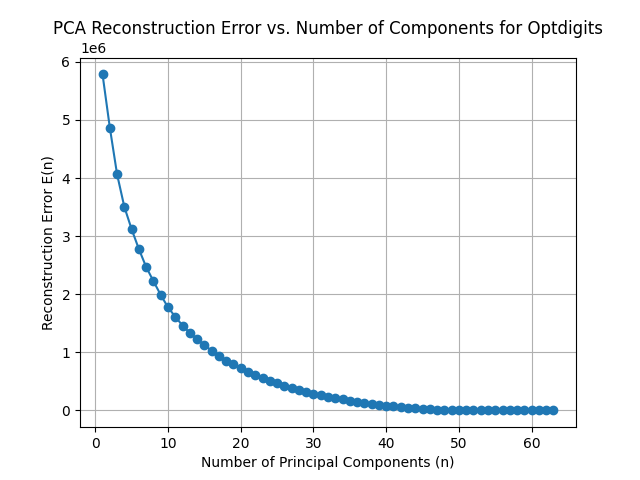
\includegraphics[width=490pt]{3_graph.png}
\end{figure} 


}

\end{document}